
This chapter will present the client - server application in which the model is utilized,
the technologies used, main use cases/features,
and the app's design and implementation.


\section{Technologies used}

Before discussing other implementation and design details,
this section will present the technologies and tools used in this paper's
application and model.

\subsection{Keras}
Keras is an intuitive API for creating deep neural networks,
whose aim is to reduce the cognitive load.
It makes one able to focus on the data,
but still being able to obtain state-of-the-art results, being used by NASA,
CERN, and many more scientific organizations due to its flexibility,
but also by the top-5 winning teams on Kaggle, due to its speed of iterations,
letting one run experiments much more straightforward.\cite{keras}

\subsection{Flask}
Flask is a WSGI web application framework designed for an easier and quicker start,
but can also scale up to complex applications,
becoming one of the most popular Python web application frameworks.\cite{flask}

Flask does not demand any dependencies,
leaving it up to the developer to choose,
based on their needs, the tools and libraries they want to use. .\cite{flask}

\subsection{React}
React is a virtual-dom javascript library used for developing user interfaces.
It is declarative, making it more manageable to create interactive UIs,
designing simple views for each state of the application,
React efficiently updating,
and re-rendering the minimum number of components when the data changes.
Being declarative views it makes the code more predictable and more comfortable
to debug.
It is component-based,
allowing encapsulating simpler components then compose them into complex UIs.

\begin{figure}[H]
  \centering
  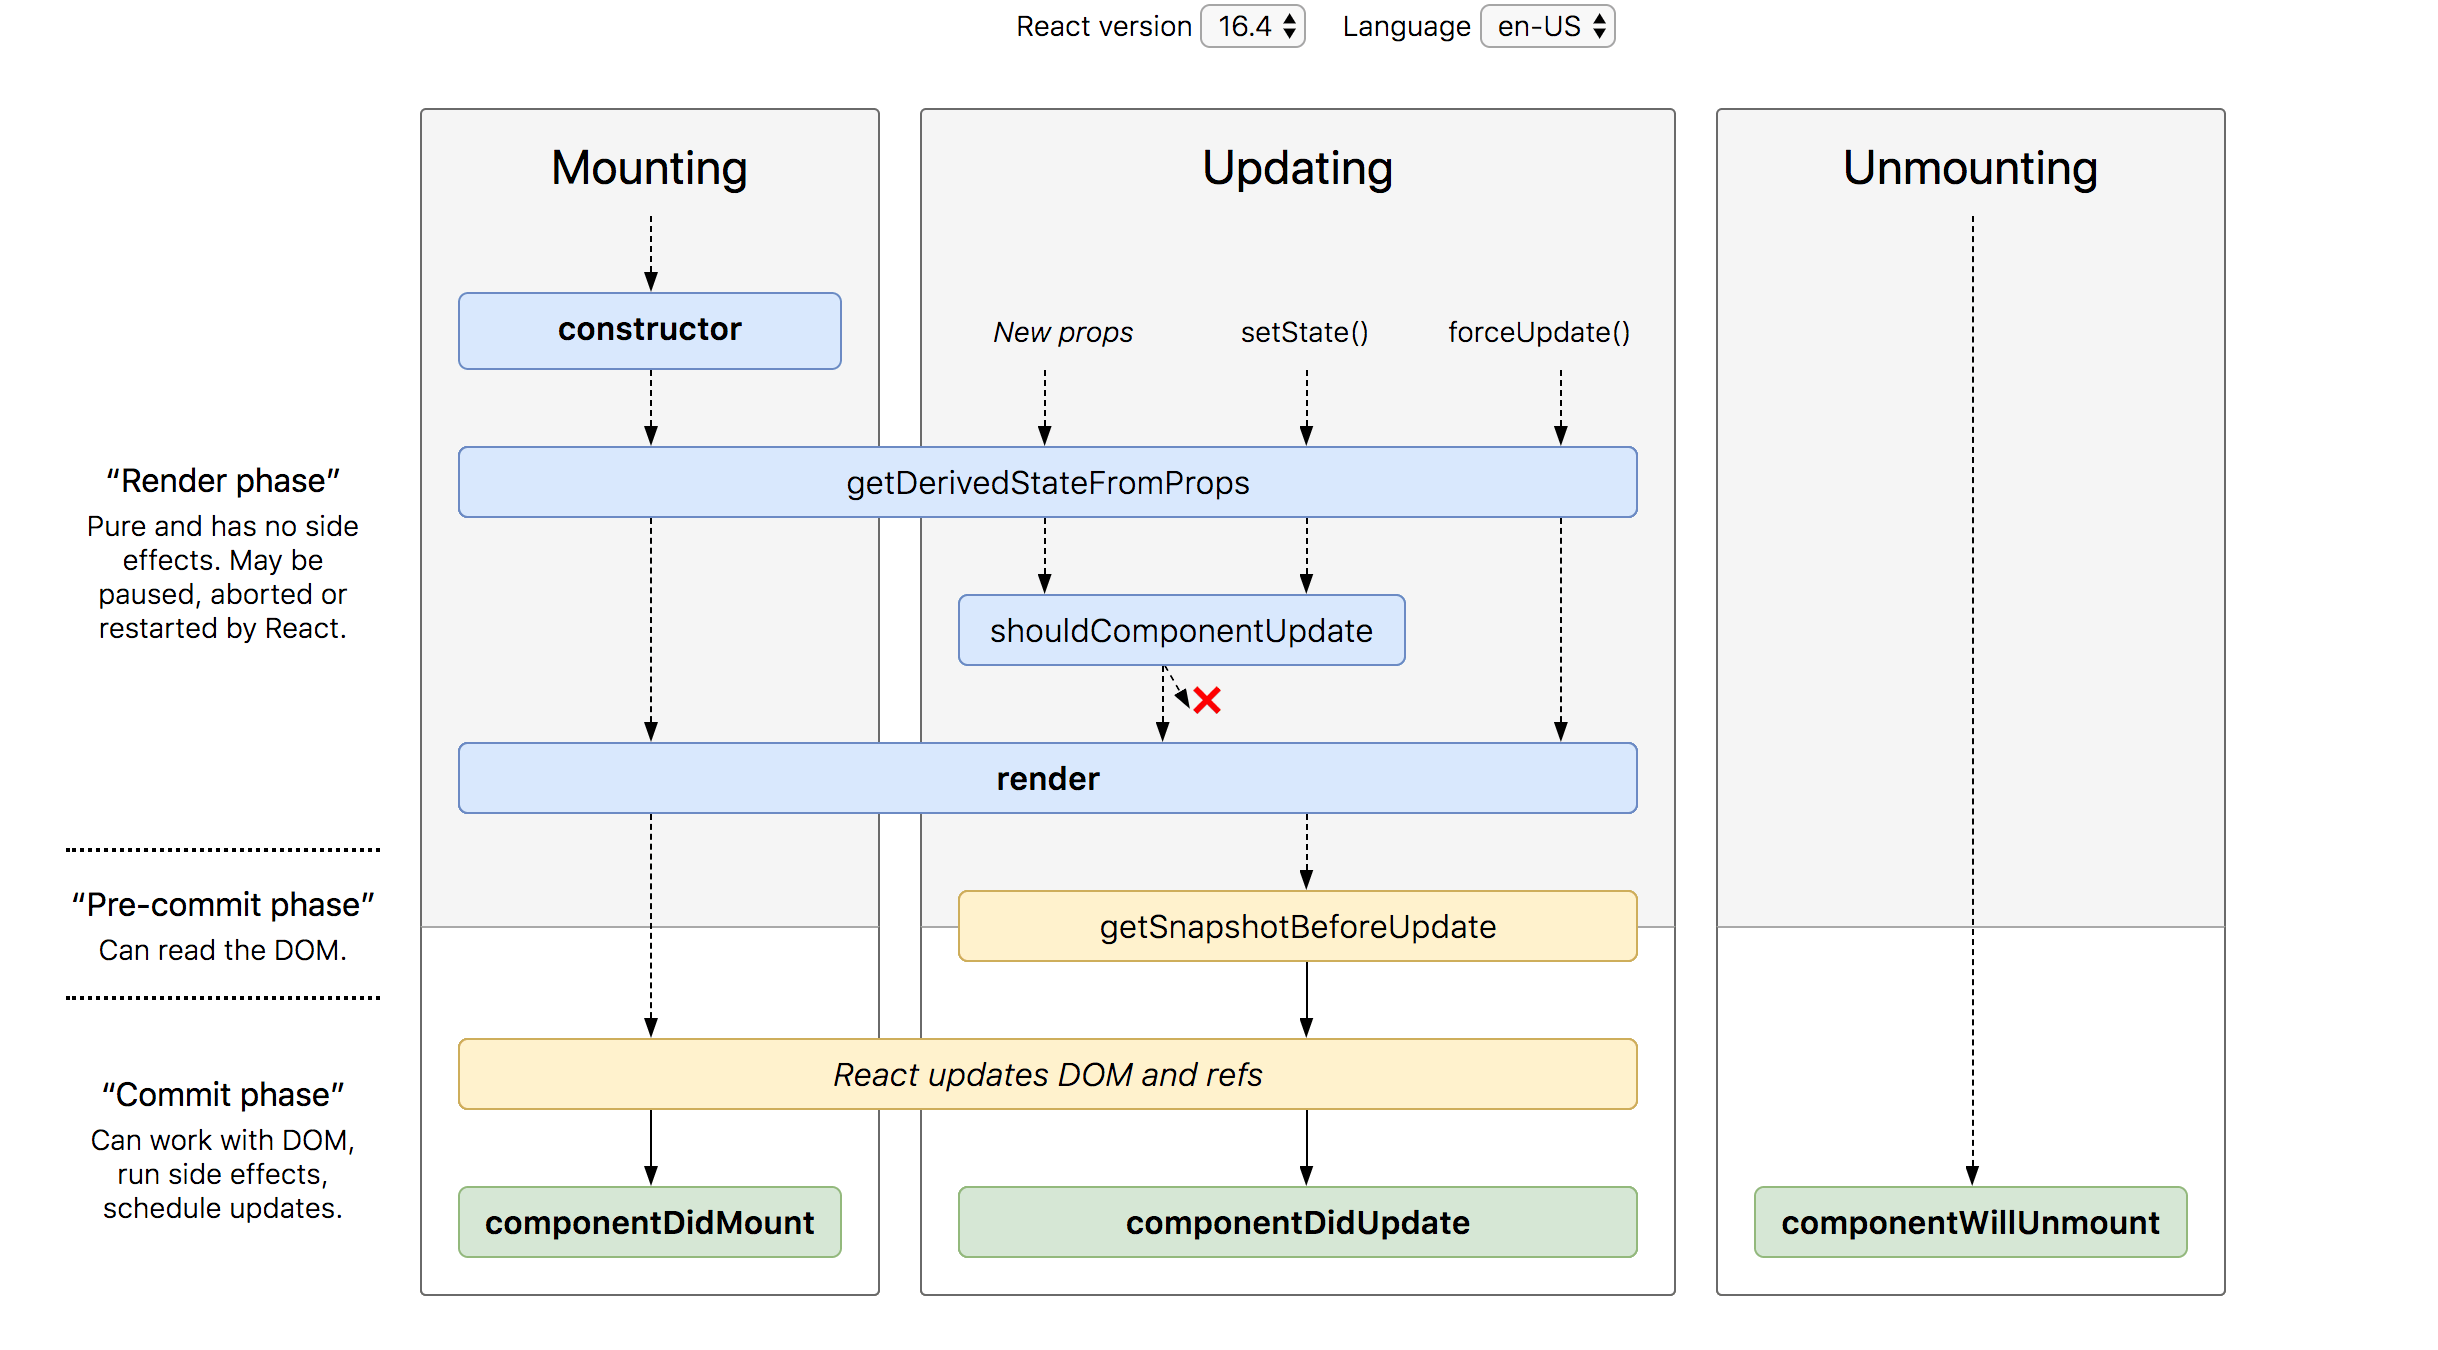
\includegraphics[width=.8\textwidth]{lifecycle}
  \caption{\emph{Lifecycle of a React Component}}
  \label{fig:lifecycle}
\end{figure}

Each created component is extending the React Component class
and should implement the render function.
It takes the input data and returns what to display.
Each component has two types of input data, which, when modified,
trigger re-rendering: props or external properties, and state or internal properties.
The rendering process is described as a lifecycle,
with a series of predefined steps,
some of them having a method that can be overridden
for a better manipulating of the UI, as seen in Figure \emph{\ref{fig:lifecycle}}.

\subsection{MobX-state-tree}
Mobx-state-tree (MST) is a state management library whose purpose
is to combine the traceability of immutable data with the simplicity
and ease of mutable data, also using the reactiveness
and performance of observable data.
The central concept of MST is the living tree.
It is an observable container data structure that consists of mutable data,
from inside the tree, using some defined methods, called actions,
from which are automatically generated immutable objects, called snapshots.
For developing the app, MST was chosen over other state management alternatives
(Redux, Flux, Recoil) thanks to its ease of writing,
lack of boiler code, and reactiveness of observable data.


\section{Main use cases/features}
In the following section,
there will be presented the main use cases of our application,
as depicted in Figure \emph{\ref{fig:usecase}}.
The main features/use cases of the app are the following:
\begin{itemize}
  \item{
        \emph{Generate song}: the musician should be able to input values
        for valence and arousal, and the app should respond with a composed song,
        that induces the corresponding emotion.
        \begin{itemize}
          \item actor: musician
          \item precondition: inputs for valence, arousal, and other model's features
          \item postcondition: a new song is generated and displayed to the user's browser
          \item path: the user should open the application, insert the input data, and the app would render the song it generated
        \end{itemize}
        }
  \item{
        \emph{See live edits of a song}: the musician should be capable of modifying the input and see live edits of the displayed song
        \begin{itemize}
          \item actor: musician
          \item precondition: a song generated before
          \item postcondition: UI is updated with the new form of the song
          \item path: the user should first generate a song then modify the input variables, and the app would render the new updated song
        \end{itemize}
        }
  \item{
        \emph{Listen to songs}: the user should be able to listen to the generated song
        \begin{itemize}
          \item actor: musician
          \item precondition: a song generated before
          \item postcondition: the application will start playing the generated song
          \item path: the user should first generate a song then press space bar, and the app would play the song
        \end{itemize}
        }
\end{itemize}

\begin{figure}[H]
  \centering
  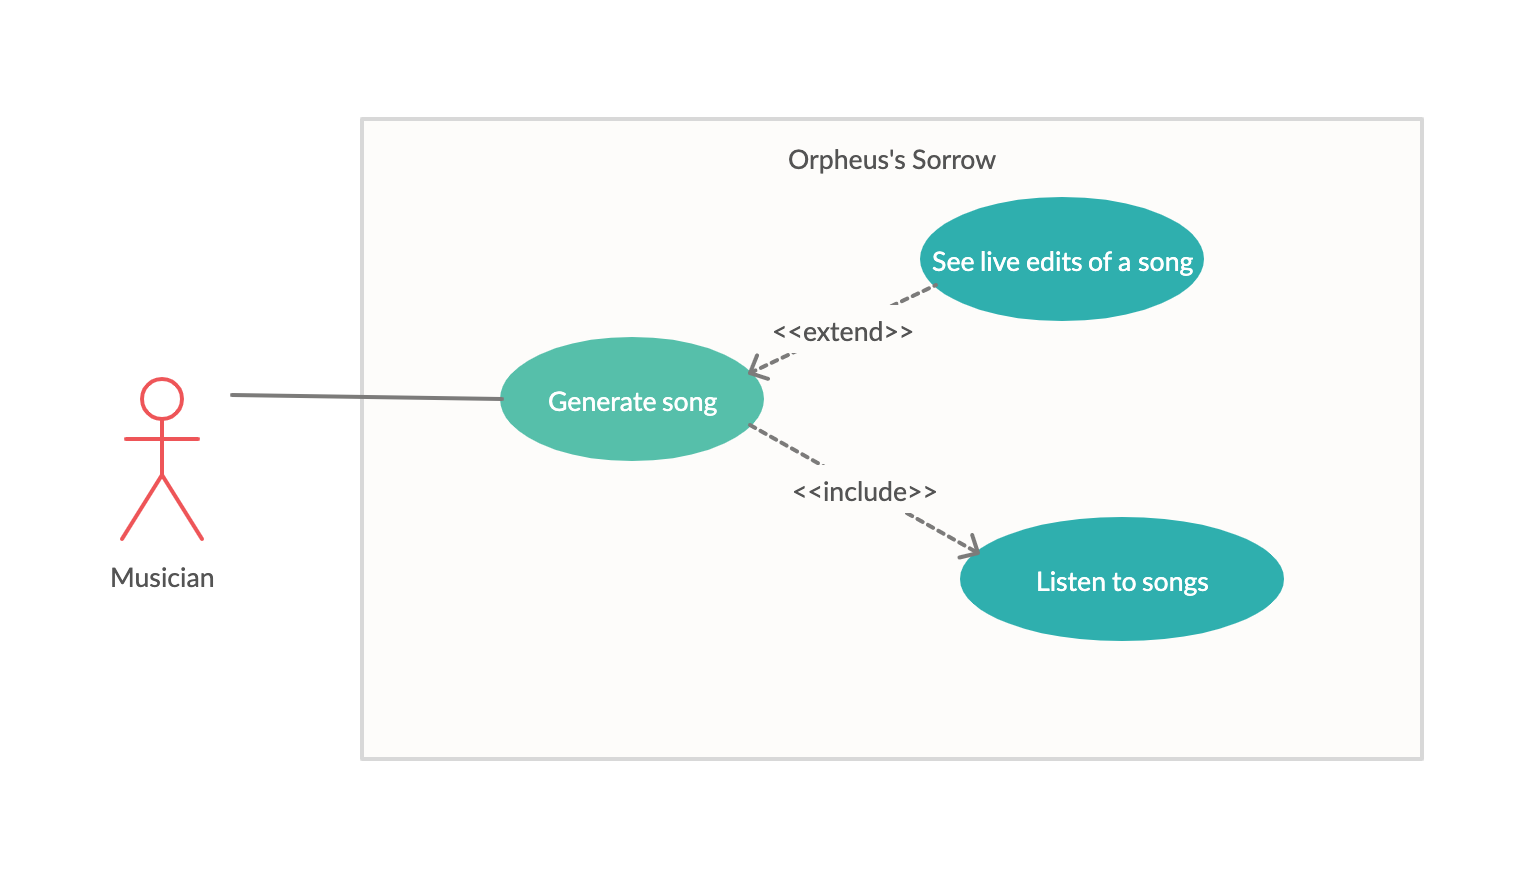
\includegraphics[width=.8\textwidth]{usecase}
  \caption{\emph{UML use case diagram for the main features}}
  \label{fig:usecase}
\end{figure}



\section{Design and implementation}

The application is composed out of two servers,
a React server for the frontend,
and a Flask server for the backend,
as shown in Figure \emph{\ref{fig:application}}.

\begin{figure}[H]
  \centering
  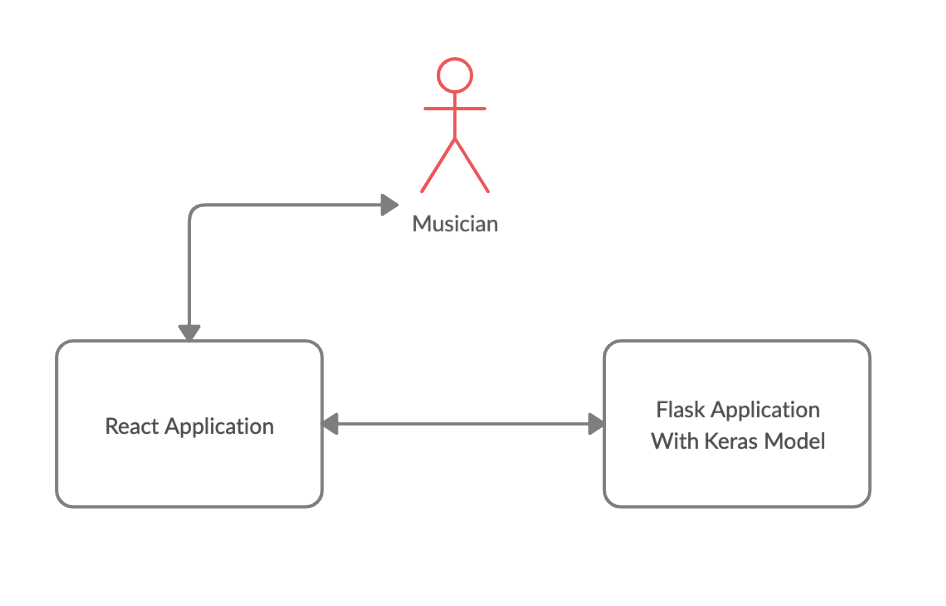
\includegraphics[width=.5\textwidth]{application}
  \caption{\emph{Main structure of the application}}
  \label{fig:application}
\end{figure}


The main aspects of the servers' design and the
interaction between the two of them or between them and
the user are visible in the sequence diagram displayed in Figure 3.
It explains how the application should react to user input,
how the data should be processed and transmitted through the servers,
considering our use cases.
The following paragraphs will present the objects composing the
diagram and the relationships between them.

\begin{figure}[H]
  \centering
  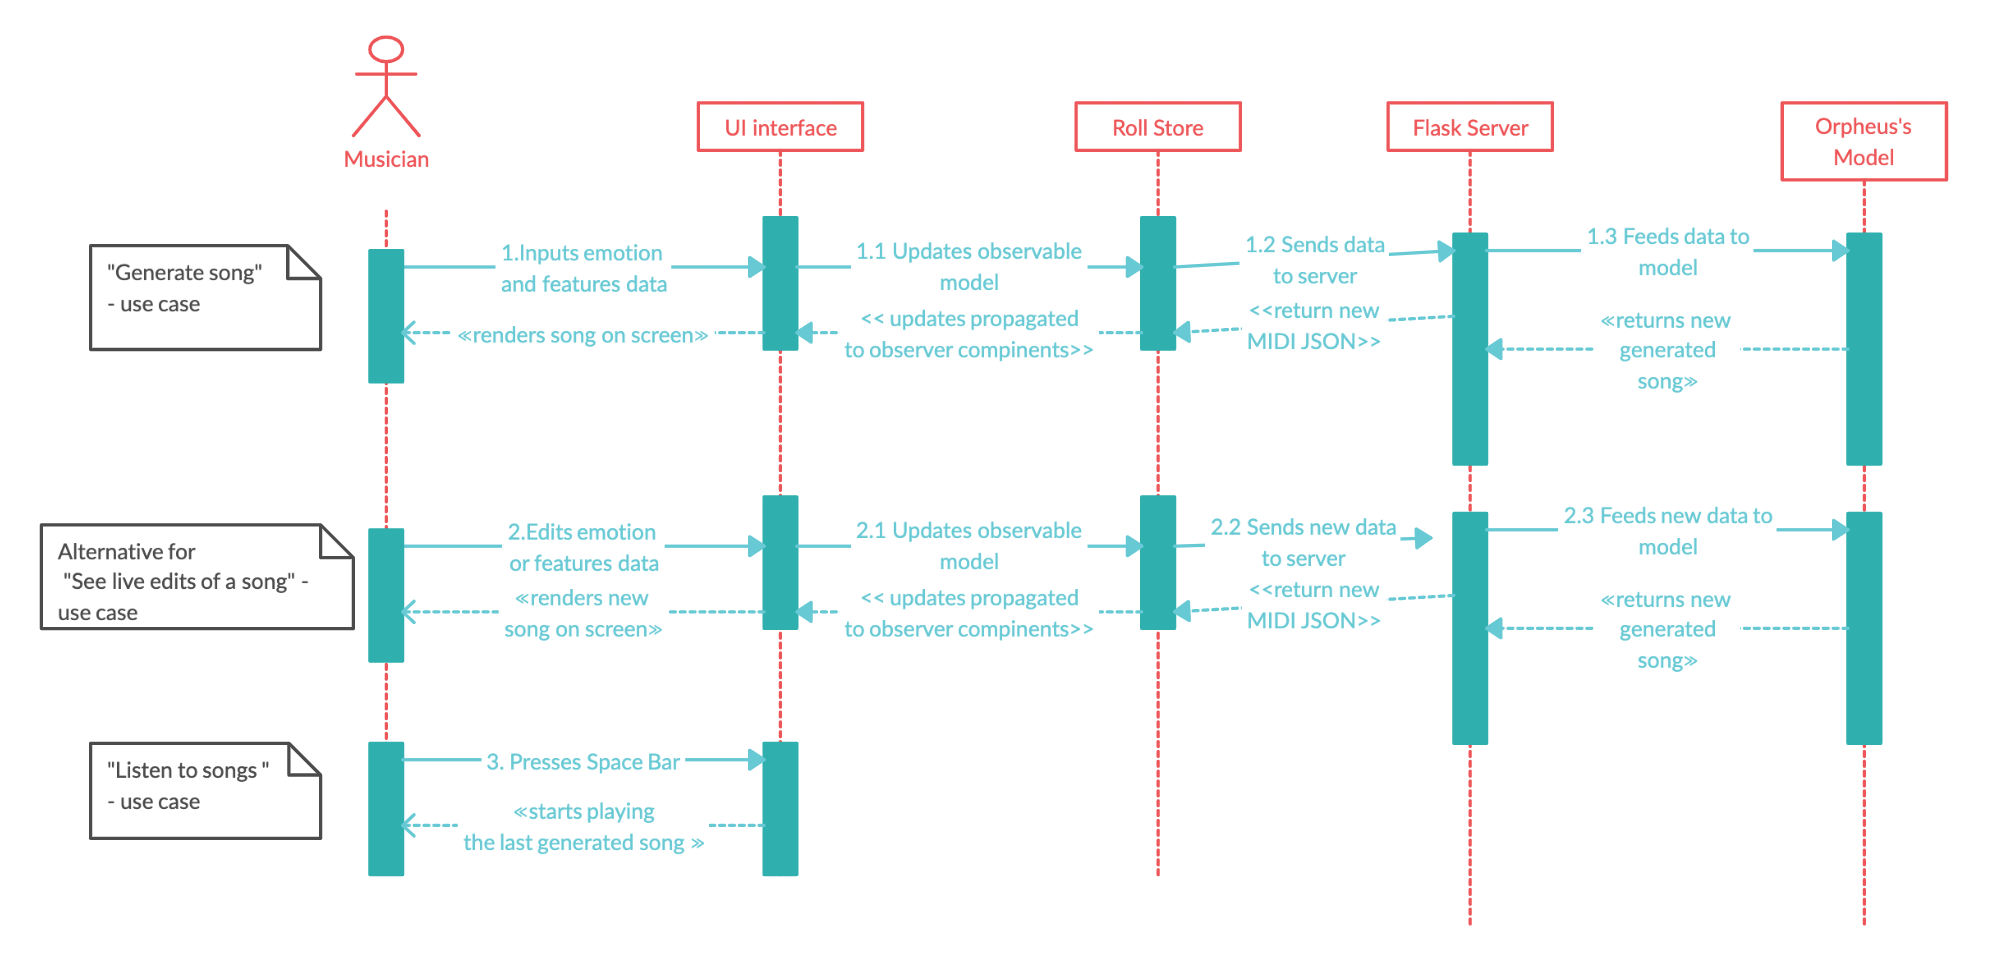
\includegraphics[width=1\textwidth]{sequence}
  \caption{\emph{UML sequence diagram containing the main use cases}}
  \label{fig:sequence}
\end{figure}


\begin{listing}
  \begin{minted}{jsx}
   // Main smart component of our application in which the store is injected
   const MidiContainer = () => {
     const { rollStore } = useStore();
     // other variables
     const memoisedSong = useMemo(() => {
       // mapping request data to our MIDI format
       const songRawBeats = rollStore.pianoRollsSnapshot.map(([roll, x, y]) => [
         roll * 96 + x,
         y + 16
       ]);
       // creating empty beats
       const songBeats = Array.from(Array((16 * 96) / 8), () => [
         [],
         [[INSTRUMENT, [], 1 / 16]]
       ]);
       // adding notes to corresponding beats
       songRawBeats.forEach(([beat, pitch]) => {
         try {
           songBeats[(beat / 8).toFixed(0)][1][0][1] = [
             ...songBeats[(beat / 8).toFixed(0)][1][0][1],
             pitch
           ];
         } catch {/* other error logic */}
       });
       return songBeats;
     }, [rollStore.pianoRollsSnapshot]);
     // Watching for `isPlaying` prop so we start playing the beat accordingly
     useEffect(() => {
       if (isPlaying) { // logic for starting the MIDI player }
       else { // logic for stopping the MIDI player }
     }, [isPlaying, memoisedSong, rollStore.volume]);
    // ... here we add other logic for our components
     return (
       <Wrapper>
         <PlayerContainer
           rolls={rollStore.pianoRollsSnapshot}
           beatIndex={midiRef.current?.beatIndex}
           ... injecting other props here
         />
        {/* other containers */}
       </Wrapper>
     );
   };
  \end{minted}
  \caption{\emph{Example of a smart component}}
  \label{lst:smart}
\end{listing}


The UI interface represents the layer the end-user,
the musician, should interact within all of the use cases.
It is build using the React library,
being composed out of function components and hooks due
to their ease of managing logic,
ease of sharing code between components, and readability.

The interface was designed using the concept of smart and presentational
components \cite{smart_dumb}. The first type refers to components that
should only be concerned about how things look (presentational)
and how to render the data they receive, as seen in Listing \emph{\ref{lst:dumb}};
they should not have any logic regarding the functionalities and
only receive callbacks. The second type defines components
that are concerned about how things work:
they provide data and behavior that is passed down
to presentational components and are linked to state management
libraries, as seen in Listing \emph{\ref{lst:smart}}.

\begin{listing}
  \begin{minted}{jsx}
/**
* Presentational component that renders all keys and positions them
* @param {number} scrollLeft -> value of the scrollLeft position
                                of the Container
*                            -> used for dynamically changing the position of
                                the keys onScroll
*/
const Keys = ({ scrollLeft }) => {
  return (
    <KeysWrapper scrollLeft={scrollLeft}>
      {NOTE_RANGE.map(item => (
        <Key key={item} isSharp={item.indexOf("#") > -1} />
      ))}
    </KeysWrapper>
  );
};
  \end{minted}
  \caption{\emph{Example of presentational component}}
  \label{lst:dumb}
\end{listing}


The Roll Store is our main state management container,
being a MobX-state-tree model,
customized for the application needs,
using the Apisauce wrapper over Axios,
a promise-based HTTP client.
It defines the structure of our data through the Mobx-based
models and the behavior/business logic through Mobx-based actions. It provides the observable data that is injected in the smart components, which, when updated, it triggers re-rendering, such that MobX alongside with React's reconciliation algorithms, reassures the minimum number of components that should update.


The Flask server is a small REST server that is mainly used
as the middleware between the client application and the
Keras model. It exposes a single REST API call,
\emph{generate\_song}, that expects to receive the
input parameters of our application;
an example of the request is the Listing 4
each parameter being explained in the following:
\begin{itemize}
  \item \emph{threshold}, the amount above the value of a generated note should be to be considered valid;
  \item \emph{valence and arousal}, the emotion data;
  \item \emph{features}, the set of the rest of 48 features that can be tweaked in our model;
  \item \emph{multiplier}, the variable used for accentuating the emotion data
\end{itemize}

Orpheus's Model represents the helper class used for creating,
training, evaluating, and loading the Keras model.
It also creates separated models for the encoder and decoder parts
for later use, when generating a new song or
normalizing and creating our metadata.

\begin{listing}[h]
  \centering
  \begin{minted}{js}
{
   "features":[
      45, 
      // ...other features, in total 48
      50
   ],
   "threshold":50,
   "valence":30,
   "arousal":29,
   "multiplier":30
}
  \end{minted}
  \caption{\emph{Example of \textbf{{get\_song}} request}}
  \label{lst:dumb}
\end{listing}

\section{User interface}

This section presents the steps for installing and running the Orpheus's Sorrow
web application on a local machine.
Then it will be discussed the interface of the app alongside the main features.

\subsection{Installation instructions}

Before downloading the application's dependencies,
some prerequisites must be installed and configured on the local machine:
\begin{itemize}
  \item \code{node}, a version above 10.x.x
  \item \code{yarn}, a version above 1.19.x, or \code{npm} above 6.x.x
  \item \code{python}, a version above 3.x with the minimum compatible \code{virtualenv}
\end{itemize}

After the mentioned requirements are satisfied,
one can download the dependencies of the projects.
For the server, one can create a virtual environment in the project's root,
using the command \code{python3 -m venv env}, \code{cd model},
and then install all the project dependencies using
the command \code{python3 -m pip install requirements.txt}.
For the client, one should open a terminal in the project's root,
\code{cd client}, run \code{yarn} (or \code{npm install}),
and wait until all the dependencies are fetched.

To run the full application,
one must run the backend first,
meaning opening a terminal in the project root, \code{cd model},
\code{python3 server.py}.
After that, the frontend can be run by also opening a terminal in the project's root,
\code{cd client}, \code{yarn start} (or \code{npm start})

\subsection{Orpheus's Sorrow interface}

The main UI of the paper's project can be seen in Figure \emph{\ref{fig:interface}}.
It is composed of two parts: the player container (the upper part),
and the input container (the bottom part).
Next, it will be discussed about each container separately.

\begin{figure}[h]
  \centering
  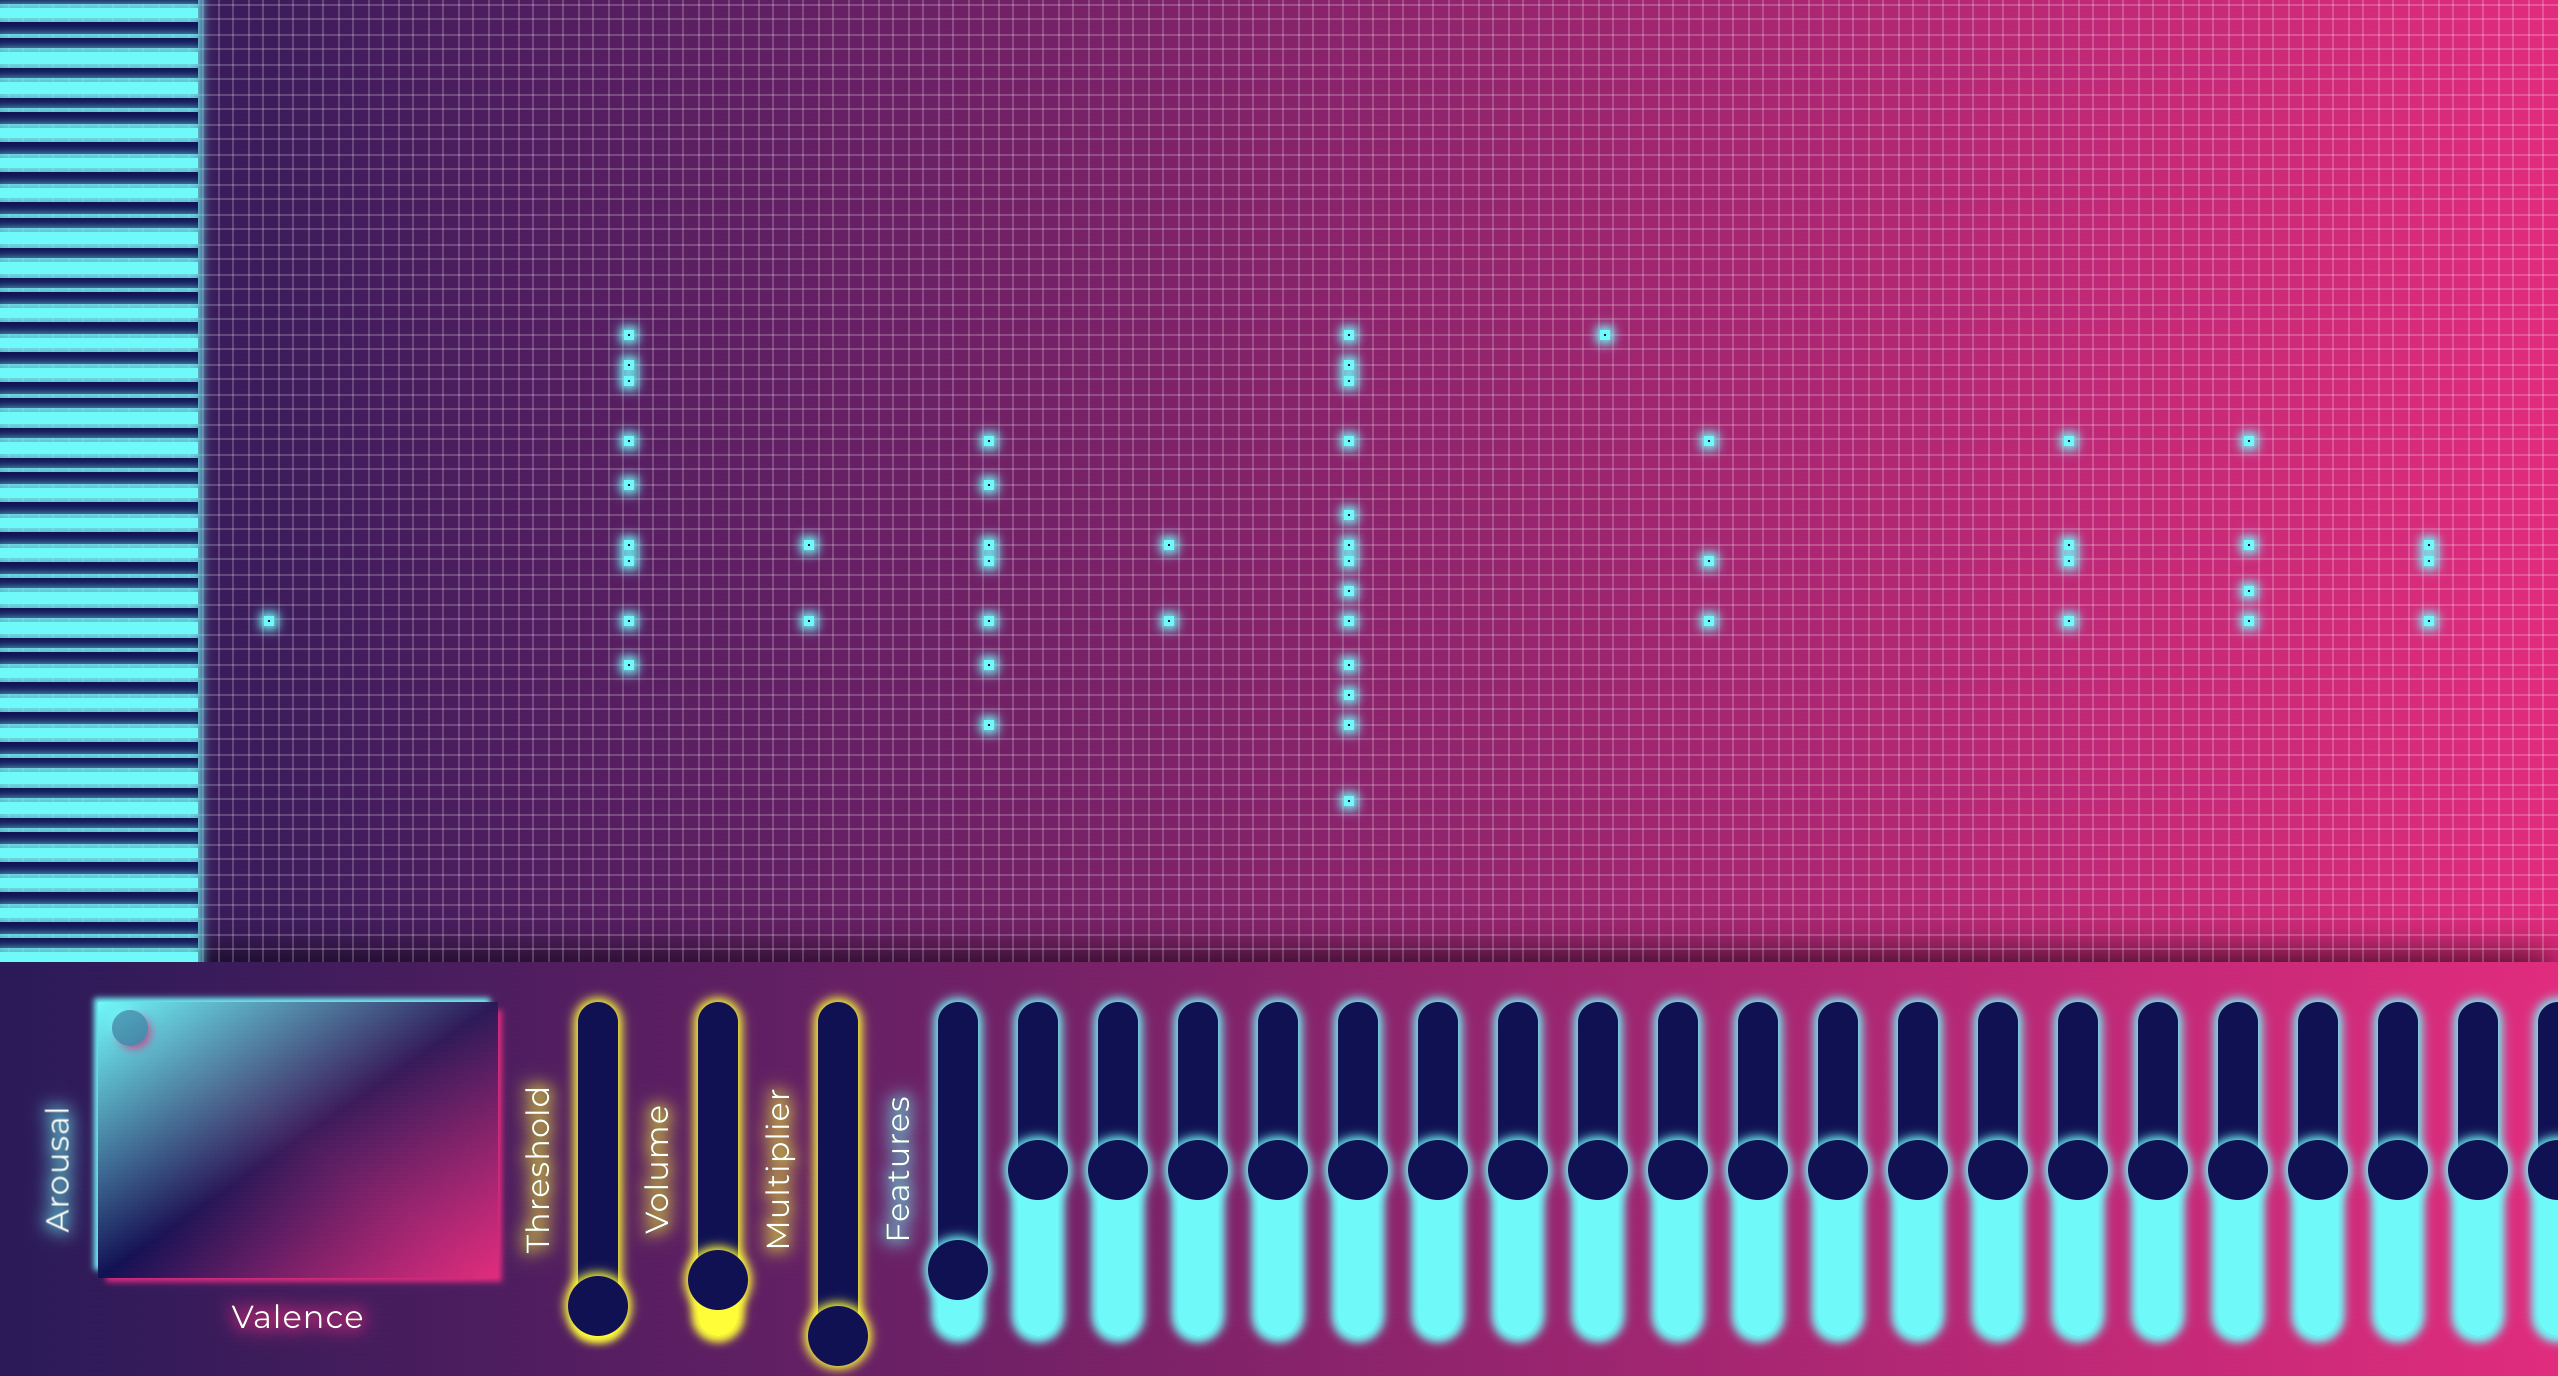
\includegraphics[width=1\textwidth]{interface}
  \caption{\emph{Orpheus's Sorrow interface}}
  \label{fig:interface}
\end{figure}


The first one, the input container,
consists of three main parts: the keys, the notes, and the grid.
The keys position matches the horizontal scroll due to the listener
on the parent container.
The notes and the grid are displayed as a piano roll,
each note being positioned at its location in time and pitch,
the main focus of the grid being to improve readability.
When pressing the spacebar,
the generated song starts playing alongside with the animation of the notes.
They are translated from right to left,
creating the illusion of the notes falling onto the keys and producing
the sound.

The second one, the bottom container,
also consists of three main parts: the emotion input, the meta-inputs,
and the feature inputs.
The emotion input is a 2d/cartesian slider with the x-axis
representing the valence value and the y-axis the arousal value.
The meta-inputs are the threshold, volume, and multiplier sliders.
The first mentioned, as discussed before,
represents the minimum value a note can have to be considered valid.
The volume slider represents the volume of the MIDI player.
When generating songs,
one could desire to amplify the values of the emotion data so the model will be more
influenced by them when composing.
Prompted by this need, the multiplier slider was introduced;
its primary purpose is to be multiplied with the valence and arousal values.
The last part contains the feature sliders that can tweak the other
variables of the features the model identified; in other words,
it changes the structure of the song that is being composed.
When modifying any of the sliders mentioned above, the song is being recomposed,
hence, the possibility to edit the song almost instantaneously,
easing the entire process, which is the principal purpose of the client app.